\documentclass[a4paper]{article}
\usepackage{pbox}
\usepackage{listings}
\usepackage{graphicx}
\usepackage{float}
\usepackage{hyperref}


\newcommand{\getAuthor}{Boris Deletic}
\newcommand{\getDoctype}{Project Plan}
\newcommand{\getTitle}{Imaging Quantum Gravity with Supercomputers}
\newcommand{\getUniversity}{University of Cambridge}
\newcommand{\getSupervisor}{\textbf{Will Barker}\\
Kavli Institute of Physics\\[1em] 
\textbf{David Yallup}\\ 
Kavli Institute of Physics}
\newcommand{\getSubmissionDate}{\today}

\begin{document}
\begin{titlepage} 
    \centering 
    
\includegraphics[height=20mm]{logo} {% 
    \vspace*{20mm} }\\
    {\large\MakeUppercase{\getUniversity{}}}\\ 
    \vspace{20mm}
    {\Large \getDoctype{}}\\
    \vspace{15mm}
    {\huge\bfseries \getTitle{}}\\
    \vspace{15mm} 
    \begin{tabular}{l l} 
        Author: & \getAuthor{} \\[1em] 
        Supervisor: & \pbox[t]{5cm}{\getSupervisor{}} \\ 
        Submission Date: & \getSubmissionDate{} \\
    \end{tabular} 
  \end{titlepage}

  \section{Introduction}
        The unification of Quantum Field Theory and General Relativity
        remains one of the largest unsolved problems in physics. One
        leading approach to developing theories of Quantum gravity
        uses computational models of lattice field theory on non-flat
        spacetimes to probe for critical points where real physics may
        arise. A promising lattice field theory (LFT) is Causal
        Dynamical Triangulation (CDT), which allows spacetime to
        evolve as a dynamical variable rather than be kept as a static
        background. \\

    A challenge with CDT is the high dimensional scaling of the
    model, making large simulations prohibitively expensive to
    run. Therefore, a carefully selected algorithm must be used to run
    the simulations in order to collect physical results and one such
    algorithm well suited for this problem is Nested
    Sampling\cite{1}. \\

    One aim of the project is to employ Nested Sampling to evolve a
    CDT model and extract observables with high precision. The initial
    problem will focus be on simple LFT models, which will present
    many challenges with using Nested Sampling. Once this has been
    acheived, the complexity of the model will gradually be increased,
    adding more elements of physics and pushing the computational
    limits. 

    Furthermore, the aim is then to produce visualisations of the Quantum
    gravity model, such as snapshots of the spacetime microstates and
    images of the different observables exploring new physics. This
    task will involve significant programming challenges in order to
    visualie higher dimensional manifolds and fractal structures.

    \section{Causal Dynamical Triangulation}
    Causal Dynamical Triangulation turns spacetime into a dynamic part of the model which can evolve according to a specified action. CDT discretises d-dimensional spacetime into a set of d-simplexes (2-simplex being a triangle) which are connected together along their edges. The triangles can switch connecting edges to create curvature in the spacetime with each configuration contributing to the Einstein-Hilbert action. 
    $$S = \frac{1}{G} \int{d^4x \sqrt{ - \det g} ( R - 2\Lambda ) } $$
    Where $G$ is the gravitational constant, $R$ is the Ricci curvature scalar computed from the triangle configuration, and $\Lambda$ is the cosmological constant. This action can then be computationally minimised to find the distribution of spacetime microstates from which physical observables can be extracted.

\begin{figure}[H]
\centering
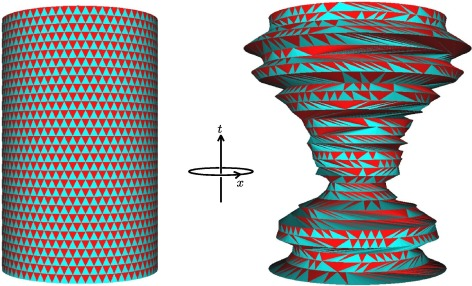
\includegraphics[width=0.75\textwidth]{cdt}
\caption{Causal Dynamical Triangulation Microstates for 1+1 spacetime
  segmented into green and red simplices. Flat
  spacetime (left) and critical spacetime (right).\cite{3}}
\end{figure}

    This approach has shown to be promising in 1+1 and 2+1 dimensions with numerical results agreeing with theoretical models. CDT solves the issue of pertubative non-renormalizability with a discretized spacetime triangulation, where the lattice can be made smaller and smaller to recover the continuous physical limit without blowing up to infinities. 

    \section{$ \phi^4$ Theory}
    The most simple field theory which is solved analytically is
    $\phi^4$ theory. This is a good starting point for research as the
    results obtained can be checked against known solutions.

    The starting point is the action for $\phi^4$ theory which is shown below
    $$S = \int{\frac{1}{2} \partial_{\mu} \phi \partial^{\mu} \phi
      -\frac{m^2}{2} \phi^2  + \frac{\lambda}{4!} \phi^4 d^4x}$$
    This action can be used to construct a path integral with the
    following general form.
    $$\mathcal{Z} = \int{ [\mathcal{D}x] e^{-\frac{i}{\hbar} S[\phi]
      } }$$
    The path integral can be interpreted as a quantum mechanical
    function which fully characterises the system. It sums the
    contributions of every field configuration weighted by the action
    of that given configuration.

    An interesting observation about this expression is the similarity
    of the action to the Boltzmann factor in thermodynamics. This
    draws analogs to using the Metropolis-Hastings (MH) algorithm,
    traditionally applied to statistical mechanics, for this application
    of lattice field theory.

    Solving $\phi^4$ theory has already been implemented in C++ using
    MH with the code and results on \url{https://github.com/BorisDeletic/QuantumGravity}.
    
    \section{Nested Sampling}
    Nested Sampling is a bayesian inference algorithm which aims to
    find a set of input parameters that maximise a general likehood function. 
    It's implementation has been
    developed largely by the Astrophysics group at Cambridge for the
    use in Cosmological models. It has many potential advantages over existing algorithms used for LFT
    simulations such as Metropolis-Hastings\cite{2} and Hybrid
    Montecarlo.

    \subsection{Metropolis-Hastings Algorithm}
    Metropolis-Hastings is a rejection based Monte Carlo Markov Chain
    (MCMC) method. The outline of the algorithm applied to $\phi^4$
    theory for example is as follows
    \begin{enumerate}
      \item Pick initial field configuration $\phi_0(x)$
      \item Generate random new field by slighting pertubing the
        previous one according to $g(\phi' | \phi_t)$
      \item Calculate the acceptance probability $A(\phi') =
        e^{-\frac{1}{\hbar}S[\phi']}$
      \item Accept or Reject new state. Generate random number $u \in
        [0,1]$. \\
        If $u < A(\phi')$ Reject the state. \\
        If $u > A(\phi')$ Accept the state, set $\phi_{t+1} = \phi'$.
        \item Repeat from step 2.
      \end{enumerate}

      
    \subsection{Topological Freezing}
    One main potential advantage is the resistance to
    topological freezing which occurs near the transition critical point, an
    effect where the system gets stuck in local minima and rejection
    rates of montecarlo methods become very high. This is a well known
    phenomenon and is an active area of research.\cite{4} Nested
    Sampling overcomes topological freezing with its use of clustering
    and bimodal exploration of a distribution.

    \subsection{NS Algorithm}
    The basic approach of the algorithm is to keep multiple instances
    of input parameters and calculate the likelihood given each set of
    inputs. The instance with the lowest likelihood is then sampled
    again subject to a hard likelihood constraint, guaranteeing the
    new instance has a greater likelihood. Iteratively repeating this
    step will cause the points to converge in parameter space around
    peaks in the likelihood function. This approach is much more
    effective at exploring bimodal distributions which are important
    for characterising phase transitions.
    
\begin{figure}[H]
\centering
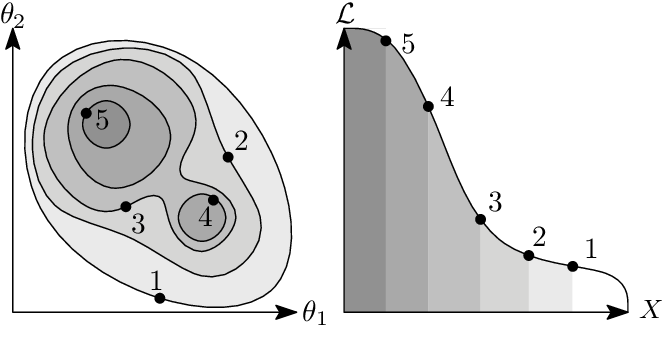
\includegraphics[width=0.75\textwidth]{ns}
\caption{Nested Sampling Bimodal Clustering. Iso-Likelihood lines in
  parameter space (left), likelihood maximisation given input
  parameters (right).}
\end{figure}

The challenges involved with applying nested sampling to lattice field theory, and
subsequently CDT will relate to the large dimensionality of the
models. Every lattice point has multiple parameters associated in the
model and must all be explored by nested sampling which itself does
not scale well with dimension.


\section{Timeline Plan}
The project aims outlined above will be acheived by completing the
following tasks with the estimated time for each goal.

\begin{enumerate}
\item Implement $\phi^4$ theory using Nested Sampling in C++. \\
  {\it 2 weeks - finish during Christmas holidays}
\item Explore dimensionality constraints of Nested Sampling and
  investigate alternate sampling schemes and their efficacy to LFT. \\
  {\it 2-4 weeks}
\item Implement CDT in nested sampling. Explore the physics of the
  model and reconcile results with literature. This is a novel piece
  of work as CDT has not been solved with Nested Sampling before. \\
  {\it 4-6 weeks}
\item Write program to visualise states and observables of
  CDT. (Additional outcome to supplement previous goals) \\
  {\it 2 weeks}
\item Extend CDT to incorporate fermionic matter and higher
  dimensional physics. (Optional if time permits) \\
  {\it 2-4 weeks}
\end{enumerate}

This plan outlines the core objectives of the project and the
estimated time to acheive them.

The main success of the project is to
demonstrate a new algorithmic approach to LFT and Quantum Gravity with Nested
Sampling. This will be a novel result which will have useful
applications to the wider community. Having physically accurate
visualisations will also provide a new useful tool for analysis of
these models which may provide a point of extension for future work. 

The extended aims provide a goal to explore new physics in addition
to the novel algorithmic research.

    
\section{Conclusion}
The application of Nested Sampling to Causal Dynamical Triangulation will be a novel computational approach to Quantum Gravity. The techniques explored will have unique advantages over current methods and will be a valuable research project for the lattice QCD and Quantum Gravity community.


\newpage
\begin{thebibliography}{9}
\bibitem{1}
W.J. Handley, M.P. Hobson, A.N. Lasenby (2015). PolyChord: next-generation nested sampling. https://arxiv.org/abs/cond-mat/9601059

\bibitem{2}
Hastings, W.K. (1970). Monte Carlo Sampling Methods Using Markov Chains and Their Applications. https://ui.adsabs.harvard.edu/abs/1970Bimka..57...97H

\bibitem{3}
Israel, Norman. (1970). Monte Carlo Sampling Methods Using Markov
Chains and Their
Applications. https://doi.org/10.1016/j.rinp.2012.10.001

\bibitem{4}
Hasenbusch, Martin. (2017). Fighting topological freezing in the two-dimensional CPN1 model. https://arxiv.org/abs/1709.09460
\end{thebibliography}

\end{document}
